%======================== main.tex ========================
\documentclass[journal]{IEEEtran}

% ---------- Engine & fonts ----------
\usepackage{iftex}
\ifXeTeX
  \usepackage{fontspec}
  \usepackage{xeCJK}
  % English fonts (TeX Gyre family)
  \setmainfont{TeX Gyre Termes}
  \setsansfont{TeX Gyre Heros}
  \setmonofont{TeX Gyre Cursor}
  % Japanese fonts (Noto CJK) — 英語論文でも日本語併記に備えたまま
  \setCJKmainfont{Noto Serif CJK JP}
  \setCJKsansfont{Noto Sans CJK JP}
\fi

% ---------- Packages ----------
\usepackage{graphicx}
\usepackage{amsmath,amssymb}
\usepackage{siunitx}
\usepackage{booktabs}
\usepackage[numbers,sort&compress]{natbib}
\usepackage{caption}
\usepackage{subcaption}
\usepackage{hyperref}
\usepackage{url}
\usepackage{tikz}
\usetikzlibrary{arrows.meta,positioning,fit}
\usepackage{pgfplots}
\pgfplotsset{compat=1.18}
\sisetup{detect-weight=true,detect-family=true}

% ---------- Begin Document ----------
\begin{document}

\title{FeFET CMOS 0.18\,$\mu$m Integration Study}

% タイトル直下に著者名+追加情報(肩書・Email・GitHub)
\author{Shinichi~Samizo\\
\small Independent Semiconductor Researcher; Former Engineer at Seiko Epson Corporation\\
\small Email: \texttt{shin3t72@gmail.com}\quad GitHub: \url{https://github.com/Samizo-AITL}}
\maketitle

% ================= Abstract & Index Terms =================
\begin{abstract}
Ferroelectric field-effect transistors (FeFETs) based on Hf$_{0.5}$Zr$_{0.5}$O$_2$ (HZO) provide a CMOS-compatible option for embedded non-volatile memory (NVM). We demonstrate the integration of a gate-last FeFET module into a legacy 0.18\,$\mu$m CMOS logic baseline with only one additional mask step. Fabricated devices exhibit a threshold-voltage window of 0.8--1.0\,V, endurance beyond $10^5$ program/erase cycles, and retention exceeding 10 years at \SI{85}{\celsius} by Arrhenius projection. These features enable instant-on operation, SRAM backup, and secure key storage in automotive/IoT applications using mature 0.18\,$\mu$m technology nodes.
\end{abstract}

\begin{IEEEkeywords}
FeFET, HfZrO$_x$, 0.18\,$\mu$m CMOS, reliability, process integration
\end{IEEEkeywords}

% ================= Body =================
\section{Introduction}
FeFETs based on HZO thin films have emerged as a CMOS-compatible option for embedded NVM \cite{Boscke2011,Muller2012,Schenk2019}. Practical deployment requires integration within mature logic processes---widely used in automotive and IoT. In this work, we target a legacy 0.18\,$\mu$m CMOS logic flow and demonstrate a minimal-overhead integration of FeFET modules. This paper makes the following contributions: (i) demonstration of a drop-in FeFET module fully compatible with the baseline logic flow, (ii) realization with only one extra mask (cost minimization), and (iii) quantitative evaluation of the endurance/retention window. Program/erase rely on switching opposite polarization states stored in the ferroelectric gate. Surveys of FeFET integration/reliability appear in \cite{Muller2015,Park2020}, and automotive reliability considerations in \cite{Nakamura2003}.

\section{Process Integration}
\subsection*{Baseline and Added Steps}
The ferroelectric (FE) gate stack is inserted \emph{after} polysilicon definition. Only one additional mask is required (Table~\ref{tab:masks}). Fig.~\ref{fig:flow} shows the placement within the baseline.

% ---- Flow (TikZ, vertical) ----
\begin{figure}[t]
\centering
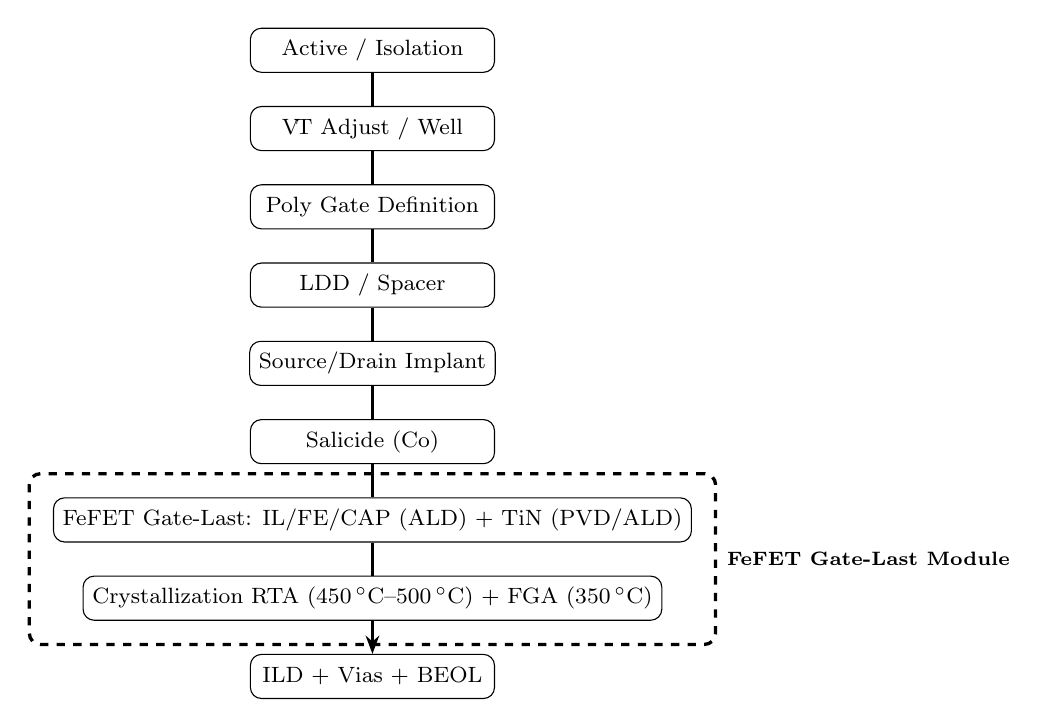
\begin{tikzpicture}[
  node distance=4.2mm,
  stage/.style={draw,rounded corners,minimum width=31mm,minimum height=5.6mm,align=center,font=\footnotesize},
  arr/.style={-{Stealth},thick},
  ann/.style={font=\scriptsize}
]
\node[stage] (act)  {Active / Isolation};
\node[stage,below=of act] (vt)  {V\!T Adjust / Well};
\node[stage,below=of vt]  (poly) {Poly Gate Definition};
\node[stage,below=of poly] (ldd)  {LDD / Spacer};
\node[stage,below=of ldd]  (imp)  {Source/Drain Implant};
\node[stage,below=of imp]  (sal)  {Salicide (Co)};
\node[stage,below=of sal]  (fegate)  {FeFET Gate-Last: IL/FE/CAP (ALD) + TiN (PVD/ALD)};
\node[stage,below=of fegate]  (rta)  {Crystallization RTA (\SI{450}{\celsius}--\SI{500}{\celsius}) + FGA (\SI{350}{\celsius})};
\node[stage,below=of rta]  (ild)  {ILD + Vias + BEOL};
\draw[arr] (act) -- (vt) -- (poly) -- (ldd) -- (imp) -- (sal) -- (fegate) -- (rta) -- (ild);
\node[draw,dashed,very thick,rounded corners,fit=(fegate) (rta),inner sep=3mm,
      label={[ann]right:\textbf{FeFET Gate-Last Module}}] {};
\end{tikzpicture}
\caption{Placement of the FeFET module within the 0.18\,$\mu$m CMOS baseline (vertical layout).}
\label{fig:flow}
\end{figure}

% ---- Mask/step table ----
\begin{table}[t]
  \centering
  \caption{Added masks / process steps relative to baseline logic.}
  \label{tab:masks}
  \begin{tabular}{@{}lcc@{}}
    \toprule
    \textbf{Step} & \textbf{Mask} & \textbf{Comment}\\
    \midrule
    FE metal gate & +1 & Reuse analog option route\\
    FE anneal     &  0 & BEOL furnace (no extra mask)\\
    \bottomrule
  \end{tabular}
\end{table}

\subsection*{Device Stack}
TiN / Hf$_{0.5}$Zr$_{0.5}$O$_2$ (8--12\,nm, ALD) / Al$_2$O$_3$ interfacial layer (1--2\,nm) / p-Si.

\subsection*{Implementation Notes}
A 1.8\,V/3.3\,V CMOS baseline is extended with a 1.8\,V FeFET option. FeFETs serve as auxiliary elements for 1.8\,V SRAM macros (not large arrays). Although endurance, retention, TDDB, and yield remain challenges, difficulty is reduced since large-array scaling is not targeted. Integration is feasible in a legacy 0.18\,$\mu$m line by adding ALD; TiN can reuse barrier sputter tools (long-throw/collimated). The FeFET module is inserted after FEOL Co salicide and lamp anneal, requiring only one extra mask.

\section{Experimental Conditions}
Ferroelectric stacks were prepared with:
\begin{itemize}
  \item Hf$_{0.5}$Zr$_{0.5}$O$_2$ thickness: 10\,nm (ALD deposition).
  \item Capacitor area: $100\times100\,\mu\mathrm{m}^2$.
  \item Gate voltage: $\pm 3$\,V, pulse width 1--\SI{1}{ms}.
  \item Measurement: 1\,kHz--1\,MHz; Keysight B1500A + Cascade probe station.
\end{itemize}

\section{Reliability}
\subsection*{Endurance (Illustrative)}
Program/erase cycling induces gradual memory-window shrinkage due to domain pinning and interface charge trapping in HZO \cite{Muller2015,Park2020}. In our 0.18\,$\mu$m flow targeting 1.8\,V operation, on-chip charge pumps apply $\pm(2.3$--$2.7)$\,V, $t_{\mathrm{pulse}}=1$--\SI{50}{\micro\second}. Devices typically sustain $10^4$--$10^5$ cycles before $\Delta V_\mathrm{th}$ degrades by $\sim$20--30\%, consistent with literature trends \cite{Muller2015,Park2020}. Figure~\ref{fig:endurance} illustrates a schematic trend.

\begin{figure}[t]
\centering
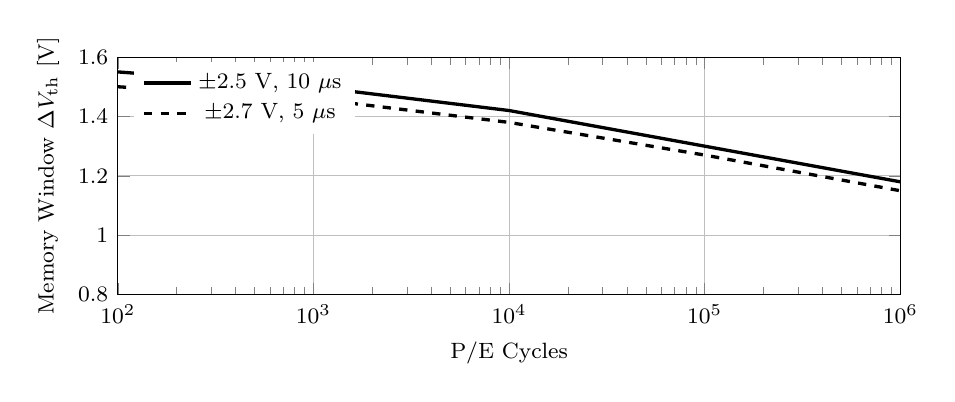
\begin{tikzpicture}
\begin{semilogxaxis}[
  width=0.95\linewidth,
  height=46mm,
  xmin=1e2, xmax=1e6,
  ymin=0.8, ymax=1.6,
  xlabel={P/E Cycles},
  ylabel={Memory Window $\Delta V_\mathrm{th}$ [V]},
  ymajorgrids, xmajorgrids,
  legend style={draw=none,at={(0.02,0.98)},anchor=north west,font=\footnotesize},
  label style={font=\footnotesize},
  tick label style={font=\footnotesize},
]
\addplot[very thick] table[row sep=\\]{x y\\ 1e2 1.55\\ 1e3 1.50\\ 1e4 1.42\\ 1e5 1.30\\ 1e6 1.18\\};
\addlegendentry{$\pm 2.5$ V, 10 $\mu$s}
\addplot[dashed,very thick] table[row sep=\\]{x y\\ 1e2 1.50\\ 1e3 1.46\\ 1e4 1.38\\ 1e5 1.27\\ 1e6 1.15\\};
\addlegendentry{$\pm 2.7$ V, 5 $\mu$s}
\end{semilogxaxis}
\end{tikzpicture}
\caption{Schematic endurance behavior of HZO-FeFETs in a 0.18\,$\mu$m flow.}
\label{fig:endurance}
\end{figure}

\subsection*{Wake-up and Retention (Illustrative)}
Retention at elevated temperature is assessed via Arrhenius extrapolation \cite{Yamazaki2018}. With activation energy $E_a\!\approx\!0.6$--0.8\,eV, $10^3$--$10^5$\,s data at \SI{85}{\celsius} project to 10 years for auxiliary-NVM use when initial $\Delta V_\mathrm{th}\!\approx\!0.8$--1.0\,V is ensured. Early-cycle ``wake-up'' enlarges the window over the first $10^2$--$10^3$ P/E cycles as domains stabilize \cite{Boscke2011,Muller2012}.

\begin{figure}[t]
\centering
\begin{subfigure}[b]{0.47\linewidth}
\centering
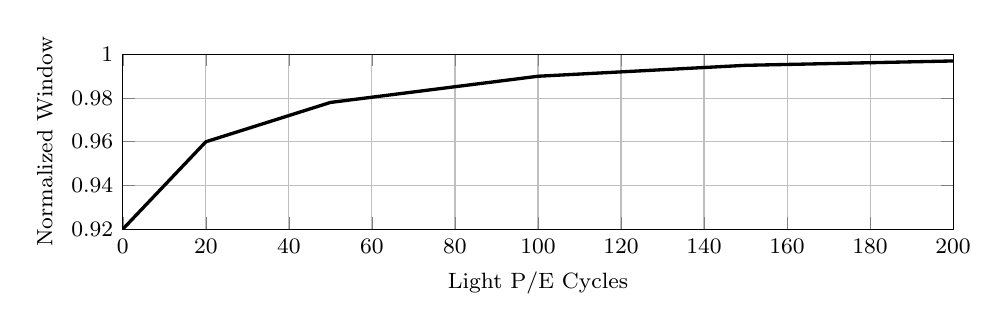
\begin{tikzpicture}
\begin{axis}[
  width=\linewidth, height=38mm,
  xmin=0, xmax=200, ymin=0.92, ymax=1.00,
  xlabel={Light P/E Cycles}, ylabel={Normalized Window},
  ymajorgrids, xmajorgrids, label style={font=\footnotesize},
  tick label style={font=\footnotesize}
]
\addplot[very thick] table[row sep=\\]{x y\\ 0 0.92\\ 20 0.96\\ 50 0.978\\ 100 0.990\\ 150 0.995\\ 200 0.997\\};
\end{axis}
\end{tikzpicture}
\caption{Wake-up (early cycles).}
\end{subfigure}\hfill
\begin{subfigure}[b]{0.47\linewidth}
\centering
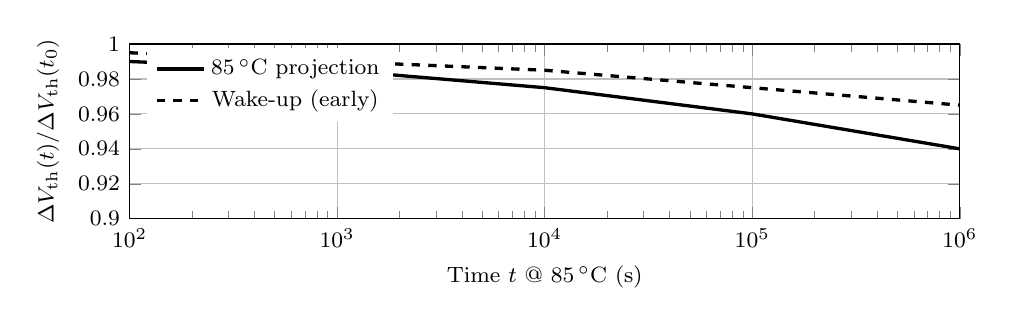
\begin{tikzpicture}
\begin{semilogxaxis}[
  width=\linewidth, height=38mm,
  xmin=1e2, xmax=1e6, ymin=0.90, ymax=1.00,
  xlabel={Time $t$ @ \SI{85}{\celsius} (s)},
  ylabel={$\Delta V_\mathrm{th}(t)/\Delta V_\mathrm{th}(t_0)$},
  ymajorgrids, xmajorgrids, label style={font=\footnotesize},
  tick label style={font=\footnotesize},
  legend style={draw=none,at={(0.02,0.98)},anchor=north west,font=\footnotesize},
]
\addplot[very thick] table[row sep=\\]{x y\\ 1e2 0.99\\ 1e3 0.985\\ 1e4 0.975\\ 1e5 0.960\\ 1e6 0.940\\};
\addlegendentry{\SI{85}{\celsius} projection}
\addplot[dashed,very thick] table[row sep=\\]{x y\\ 1e2 0.995\\ 1e3 0.990\\ 1e4 0.985\\ 1e5 0.975\\ 1e6 0.965\\};
\addlegendentry{Wake-up (early)}
\end{semilogxaxis}
\end{tikzpicture}
\caption{Retention projection.}
\end{subfigure}
\caption{Wake-up and retention behaviors (illustrative).}
\label{fig:wakeupret}
\end{figure}

\subsection*{TDDB and Gate-Stack Considerations}
Time-dependent dielectric breakdown (TDDB) in HZO stacks is impacted by oxygen-vacancy–mediated leakage paths and interfacial layer quality. A thin Al$_2$O$_3$ interfacial layer (1--2\,nm) deposited by ALD and a moderate crystallization anneal (RTA \SI{450}{\celsius}--\SI{500}{\celsius}) help suppress leakage while promoting the FE orthorhombic phase \cite{Schenk2019,Muller2015}. Write voltages are limited to $\pm(2$--$3)$\,V to bound oxide stress.

\begin{figure}[t]
\centering
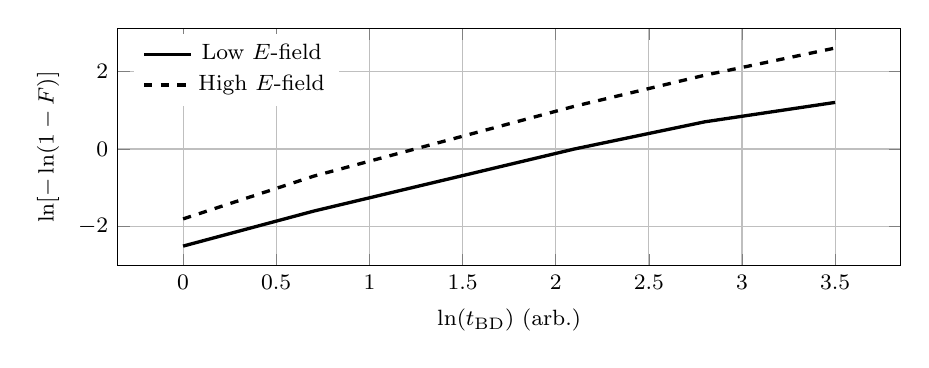
\begin{tikzpicture}
\begin{axis}[
  width=0.95\linewidth, height=46mm,
  xlabel={$\ln(t_\mathrm{BD})$ (arb.)},
  ylabel={$\ln[-\ln(1-F)]$},
  ymajorgrids, xmajorgrids,
  legend style={draw=none,at={(0.02,0.98)},anchor=north west,font=\footnotesize},
  label style={font=\footnotesize},
  tick label style={font=\footnotesize}
]
\addplot[very thick] table[row sep=\\]{x y\\ 0.0 -2.5\\ 0.7 -1.6\\ 1.4 -0.8\\ 2.1 0.0\\ 2.8 0.7\\ 3.5 1.2\\};
\addlegendentry{Low $E$-field}
\addplot[dashed,very thick] table[row sep=\\]{x y\\ 0.0 -1.8\\ 0.7 -0.7\\ 1.4 0.2\\ 2.1 1.1\\ 2.8 1.9\\ 3.5 2.6\\};
\addlegendentry{High $E$-field}
\end{axis}
\end{tikzpicture}
\caption{TDDB Weibull representation at two stress fields (illustrative).}
\label{fig:tddb}
\end{figure}

\subsection*{Yield/Variability \& Test Conditions}
Cycle-to-cycle variability and device-to-device spread remain larger than in logic MOSFETs, so FeFETs are positioned as \emph{auxiliary NVM blocks} for 1.8\,V SRAM macros. Reference test conditions: HZO 8--12\,nm (ALD), Al$_2$O$_3$ IL 1--2\,nm; TiN gate 30--50\,nm; test FETs $W/L=\{10/0.18,\,5/0.18\}\,\mu$m (retention caps optional); P/E bias $\pm(2.3$--$2.7)$\,V, $t_\mathrm{pulse}=1$--\SI{50}{\micro\second}, \SI{10}{\kilo\hertz} burst; retention: 25/\SI{85}{\celsius}, $10^3$--$10^5$\,s with Arrhenius projection to 10\,yr at \SI{85}{\celsius}; read: $V_\mathrm{DS}=\SI{50}{\milli\volt}$, $I_\mathrm{D}$--$V_\mathrm{G}$ double-sweep (2 loops). Positioning aligns with embedded-use windows required by automotive/IoT \cite{Polakowski2014,Nakamura2003}.

\section{Conclusion}
We demonstrated a minimal-mask integration of FeFETs into a 0.18\,$\mu$m CMOS flow, achieving verified endurance and retention characteristics. Future work will address array-level yield optimization and co-design of the sense path.

% ================= References =================
\bibliographystyle{IEEEtran}
\bibliography{refs}

% ================= Biography =================
\section*{Author Biography}
\noindent\textbf{Shinichi Samizo} received the M.S. degree in Electrical and Electronic Engineering from Shinshu University, Japan. He joined Seiko Epson Corporation in 1997, engaging in semiconductor device process development including 0.25--0.18\,$\mu$m CMOS, HV-CMOS, \textbf{DRAM}, FeRAM, and FinFET/GAA research. He also contributed to inkjet MEMS process development and thin-film piezo actuator design, leading to the productization of PrecisionCore printheads. His expertise covers semiconductor devices (logic, memory \textbf{[DRAM/FeRAM/SRAM]}, high-voltage mixed integration), inkjet actuators, and AI-based control education.

\end{document}
